\subsection{Tiling puzzle and Z3 SMT solver}

This is classic problem: given 12 polyomino titles, cover mutilated chessboard with them (it has 60 squares with no central 4 squares).

The problem is covered at least in \href{https://arxiv.org/pdf/cs/0011047.pdf}{Donald E. Knuth - Dancing Links},
and this Z3 solution has been inspired by it.

Another thing I've added: graph coloring. You see, my script gives correct solutions, but somewhat unpleasant visually.
So I used colored pseudographics. There are 12 tiles, it's not a problem to assign 12 colors to them.
But there is another heavily used SAT problem: graph coloring.

Given a graph, assign a color to each vertex/node, so that colors wouldn't be equal in adjacent nodes.
The problem can be solved easily in SMT: assign variable to each vertex.
If two vertices are connected, add a constraint: \textit{vertex1\_color != vertex2\_color}.
As simple as that.
In my case, each polynomio is vertex and if polyomino is adjacent to another polyomino, an edge/link is added between vertices.
So I did, and output is now colored.

But this is planar graph (i.e., a graph which is, if represented in two-dimensional space has no intersected edges/links).
And here is a famous four color theorem can be used.
The solution of tiled polynomios is in fact like planar graph, or, a map, like a world map.
Theorem states that any planar graph (or map) can be colored only 4 colors.

This is true, even more, several tilings can be colors with only 3 colors:

\begin{figure}[H]
\centering
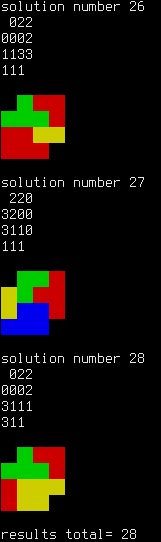
\includegraphics[scale=1]{SMT/tiling/small.png}
\caption{}
\end{figure}

Now the classic: 12 pentominos and "mutilated" chess board, several solutions:

% TODO side by side in table:
\begin{figure}[H]
\centering
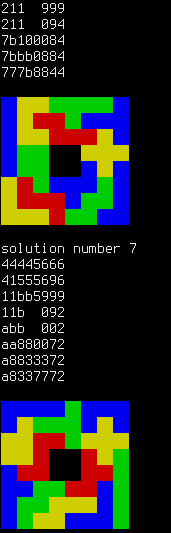
\includegraphics[scale=1]{SMT/tiling/big1.png}
\caption{}
\end{figure}

\begin{figure}[H]
\centering
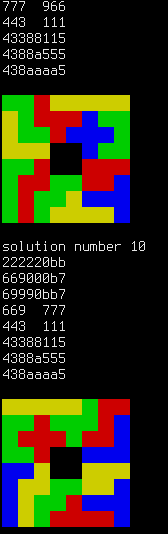
\includegraphics[scale=1]{SMT/tiling/big2.png}
\caption{}
\end{figure}

% FIXME URL
The source code: \url{https://github.com/DennisYurichev/yurichev.com/blob/master/blog/tiling_Z3/tiling.py}.

Further reading: \url{https://en.wikipedia.org/wiki/Exact_cover#Pentomino_tiling}.

Four-color theorem has an interesting story, it has been finally proved in 2005 by Coq proof assistant:
\url{https://en.wikipedia.org/wiki/Four_color_theorem}.

